\textbf{\Large Grundlagen}\\

Das ventilatorische Schwellenkonzept basiert auf der physiologischen Reaktion des Körpers auf die zunehmende Belastung bei einer Spiroergometrie. Da der Muskelgehalt des körpereigenen Energiestoffs ATP zur Muskelkontraktion nur für eine kurze Zeit ausreicht, muss dieser für andauernde Arbeit durch Glykolyse oxidativ resynthetisiert werden \cite{Kroidl.2015}. Reicht ab einer bestimmten Belastung die Sauerstoffaufnahme (\.{V}O\textsubscript{2}) nicht mehr aus, funktionieren gewisse Coenzyme nicht mehr, sodass in den Muskeln Laktat akkumuliert und es allmählich zur metabolischen Azidose (Übersäuerung) kommt. Der Körper versucht, dies durch Puffer-Reaktionen zu kompensieren, wodurch überschüssiges Kohlenstoffdioxid (CO\textsubscript{2}) anfällt, welches abgeatmet wird und respiratorisch gemessen werden kann.\\
Nach einer Spiroergometrie werden bestimmte Atemparameter grafisch verglichen, um ventilatorische Reaktionen auf metabolische Prozesse zu detektieren. Die sogenannten ventilatorischen Schwellen stellen Stoffwechselübergänge dar, anhand derer mit verschiedenen Modellen Trainingsbereiche bestimmbar sind. Die VT1 kann mittels der V-Slope-Methode oder anhand des Sauerstoff-Äquivalents (EQO\textsubscript{2}) grafisch identifiziert werden. Das Kohlenstoffdioxid-Äquivalent (EQCO\textsubscript{2}) oder der Vergleich der Ventilation (\.{V}E) mit der Kohlenstoffdioxidabgabe (\.{V}CO\textsubscript{2}) eignen sich zur Bestimmung der VT2.\\

\begin{picture}(\spaltenbreite,6)
\put(0.5,2){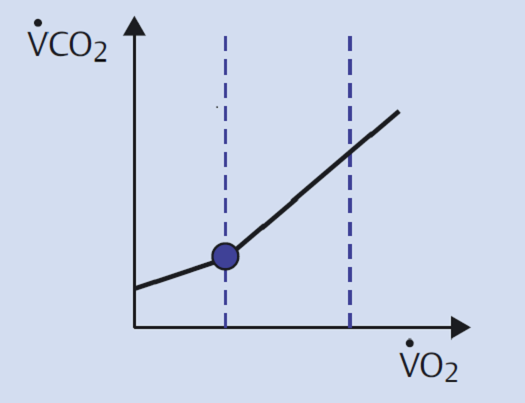
\includegraphics[width=50mm]{Bilder/vslope.png}}
\put(0.4,0.7){\parbox{720pt}{{\bf \small Abb. 1:} \small V-Slope}}
\put(6.7,2){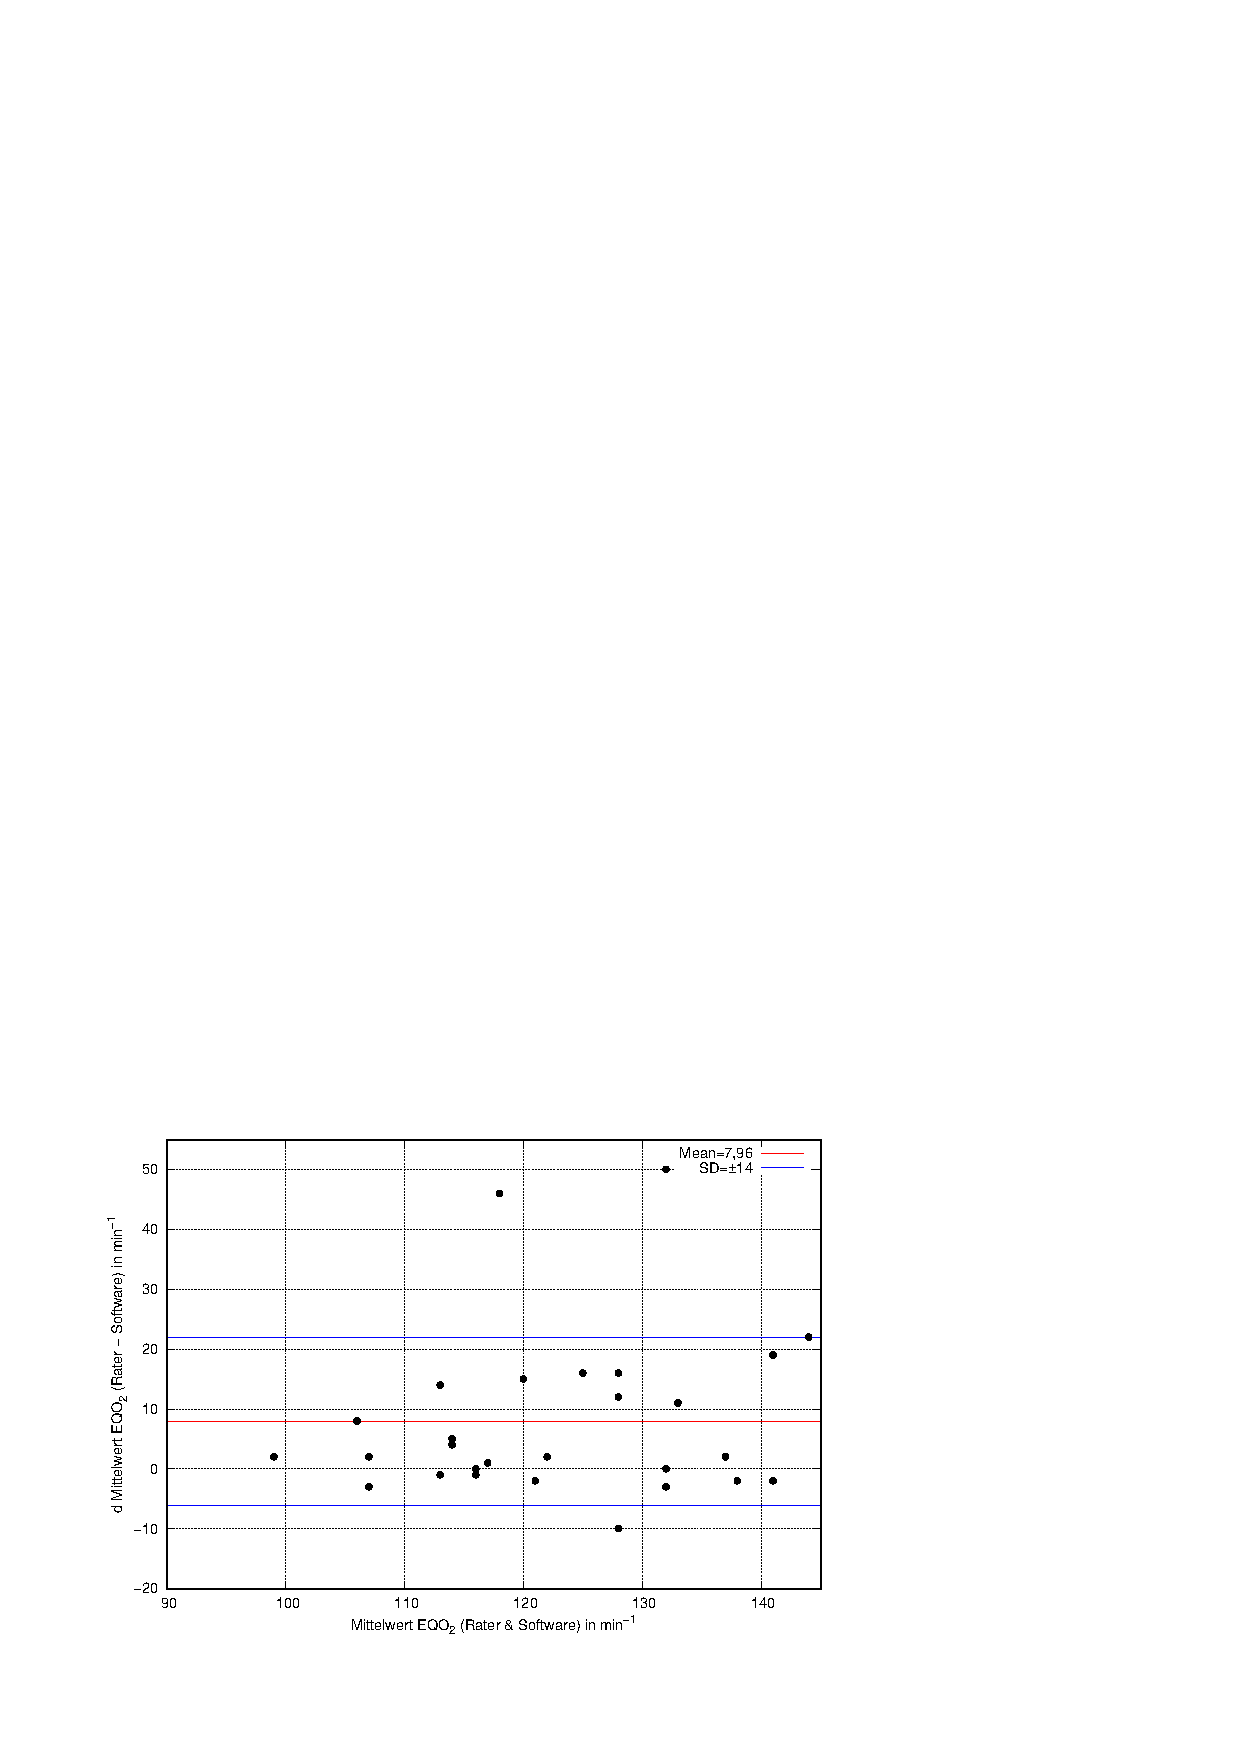
\includegraphics[width=50mm]{Bilder/eqo2.png}}
\put(6.9,0.7){\parbox{720pt}{{\bf \small Abb. 2:} \small EQO\textsubscript{2}}}
\put(12.9,2){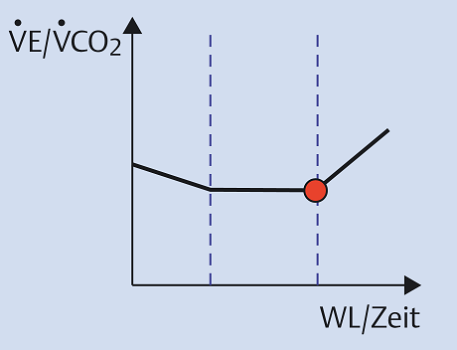
\includegraphics[width=50mm]{Bilder/eqco2.png}}
\put(12.9,0.7){\parbox{720pt}{{\bf \small Abb. 3:} \small EQCO\textsubscript{2}}}
\put(19.2,2){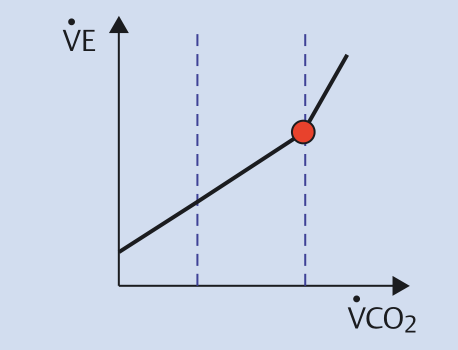
\includegraphics[width=50mm]{Bilder/field4.png}}
\put(18.9,0.78){\parbox{720pt}{{\bf \small Abb. 4:} \small \.{V}E/\.{V}CO\textsubscript{2}}}
\end{picture}
